\chapter{Frequently Asked Questions}

\section{Bordje problemen}

Het aansluiten van het bordje kan soms lastig zijn. Hieronder een aantal tips: \\

\noindent \textbf{USB kabel} \\

Voor het aansluiten van het bordje heb je een USB-A naar micro-USB kabel nodig. Sommige van deze kabels zullen niet werken, deze leveren bijvoorbeeld wel stroom naar geen date. Als het bordje niet werkt,bijvoorbeeld als hij wel aan gaat maar windows geen verbinding kan maken, probeer dan dus eerst altijd een andere kabel. Pas na 3 kabeltjes kan je met enige zekerheid zeggen dat je dit probleem hebt verholpen. \\

\noindent \textbf{Anti virus} \\

Sommige anti-virus software blokkeren USB apparaten. Probeer dus ook eens je bordje aan te sluiten terwijl je anti-virus programma uit staat.\\

\noindent \textbf{Bordje niet gevonden} \\

Het kan zijn dat de verkeerde bootloader op het bordje staat. Volg de stappen in het hoofdstuk bordje updaten om de bootloader te updaten en CirquitPython op het bordje te zetten. \\

\url{https://circuitpython.org/board/metro_m4_airlift_lite/}

\clearpage
\newpage

\section{Code Problemen}

Bij het coderen kunnen veel fouten krijgen. Een computer (en dus ook het bordje) werkt alleen als de code erop foutloos is. \\

Let bij het schrijven van het programma op het volgende: \\

\noindent \textbf{Serial en Code check} \\

In MU zitten de 'Serial (of REPL)' en 'Code Check' knoppen. Hiermee kan je goed  controleren of er fouten in je code zitten. De Serial knop geeft in een schermpje onderaan aan welke fouten er in je code zitten, hierbij staat ook op welke regel zich de fout bevind. De Code Check knop controleert de code tussen de code door. \\

\begin{figure}[h!]
    \centering
    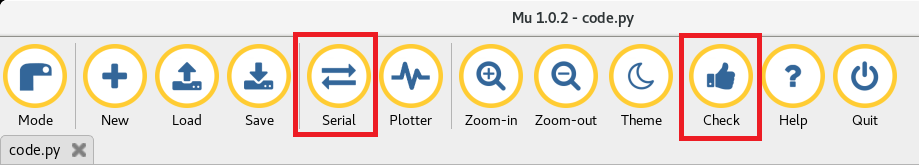
\includegraphics{figures/check.png}
    \caption{Serial en Code Check}
    \label{fig:my_label}
\end{figure}

\noindent \textbf{Code problemen} \\

\noindent Kom je er niet uit ? check dan het volgende lijstje: \\

\begin{itemize}
    \item Heet het bestand op het bordje code.py ?
    \item Staat jou code.py bestand op het bordje ?
    \item Staat jou code in het bestand code.py ?
    \item Zitten er typ fouten in je code ?
    \item Staan er onnodige spaties of hoofdletters in je code ?
    \item Stuur je de poorten aan die je wilt gebruiken ?
\end{itemize}